\documentclass{article}
% Change "article" to "report" to get rid of page number on title page
\usepackage{amsmath,amsfonts,amsthm,amssymb}
\usepackage{setspace}
\usepackage{fancyhdr}
\usepackage{lastpage}
\usepackage{extramarks}
\usepackage{chngpage}
\usepackage{soul}
\usepackage[usenames,dvipsnames]{color}
\usepackage{graphicx,float,wrapfig}
\usepackage{ifthen}
\usepackage{listings}
\usepackage{courier}


%   !!!!!!!!!!!!!!!!!!!!!!!!!!!!!!!!!!!!!!!!!!!!!!!!!!!!!
%
%   Here put your info (name, due date, title etc).
%   the rest should be left unchanged.
%
%
%
%   !!!!!!!!!!!!!!!!!!!!!!!!!!!!!!!!!!!!!!!!!!!!!!!!!!!!!


% Homework Specific Information
\newcommand{\hmwkTitle}{}
\newcommand{\hmwkSubTitle}{LU decomposition}
\newcommand{\hmwkDueDate}{May 04, 2023}
\newcommand{\hmwkClass}{Computational Physics III}
\newcommand{\hmwkClassTime}{}
%\newcommand{\hmwkClassInstructor}{Prof. Oleg Yazyev}
\newcommand{\hmwkAuthorName}{Salomon Guinchard}
\newcommand{\beq}{\begin{equation}}
\newcommand{\eeq}{\end{equation}}
\graphicspath{{./Illustrations/}{./IllustrationsResults/}}  
%
%


% In case you need to adjust margins:
\topmargin=-0.45in      %
\evensidemargin=0in     %
\oddsidemargin=0in      %
\textwidth=6.5in        %
\textheight=9.5in       %
\headsep=0.25in         %

% This is the color used for  comments below
\definecolor{MyDarkGreen}{rgb}{0.0,0.4,0.0}

% For faster processing, load Matlab syntax for listings
\lstloadlanguages{Matlab}%
\lstset{language=Matlab,                        % Use MATLAB
        frame=single,                           % Single frame around code
        basicstyle=\small\ttfamily,             % Use small true type font
        keywordstyle=[1]\color{Blue}\bf,        % MATLAB functions bold and blue
        keywordstyle=[2]\color{Purple},         % MATLAB function arguments purple
        keywordstyle=[3]\color{Blue}\underbar,  % User functions underlined and blue
        identifierstyle=,                       % Nothing special about identifiers
                                                % Comments small dark green courier
        commentstyle=\usefont{T1}{pcr}{m}{sl}\color{MyDarkGreen}\small,
        stringstyle=\color{Purple},             % Strings are purple
        showstringspaces=false,                 % Don't put marks in string spaces
        tabsize=3,                              % 5 spaces per tab
        %
        %%% Put standard MATLAB functions not included in the default
        %%% language here
        morekeywords={xlim,ylim,var,alpha,factorial,poissrnd,normpdf,normcdf},
        %
        %%% Put MATLAB function parameters here
        morekeywords=[2]{on, off, interp},
        %
        %%% Put user defined functions here
        morekeywords=[3]{FindESS, homework_example},
        %
        morecomment=[l][\color{Blue}]{...},     % Line continuation (...) like blue comment
        numbers=left,                           % Line numbers on left
        firstnumber=1,                          % Line numbers start with line 1
        numberstyle=\tiny\color{Blue},          % Line numbers are blue
        stepnumber=1                        % Line numbers go in steps of 5
        }

% Setup the header and footer
\pagestyle{fancy}                                                       %
\lhead{\hmwkAuthorName}                                                 %
%\chead{\hmwkClass\ (\hmwkClassInstructor\ \hmwkClassTime): \hmwkTitle}  %
\rhead{\hmwkClass\ : \hmwkTitle}  %
%\rhead{\firstxmark}                                                     %
\lfoot{\lastxmark}                                                      %
\cfoot{}                                                                %
\rfoot{Page\ \thepage\ of\ \protect\pageref{LastPage}}                  %
\renewcommand\headrulewidth{0.4pt}                                      %
\renewcommand\footrulewidth{0.4pt}                                      %

% This is used to trace down (pin point) problems
% in latexing a document:
%\tracingall

%%%%%%%%%%%%%%%%%%%%%%%%%%%%%%%%%%%%%%%%%%%%%%%%%%%%%%%%%%%%%
% Some tools
\newcommand{\enterProblemHeader}[1]{\nobreak\extramarks{#1}{#1 continued on next page\ldots}\nobreak%
                                    \nobreak\extramarks{#1 (continued)}{#1 continued on next page\ldots}\nobreak}%
\newcommand{\exitProblemHeader}[1]{\nobreak\extramarks{#1 (continued)}{#1 continued on next page\ldots}\nobreak%
                                   \nobreak\extramarks{#1}{}\nobreak}%

\newlength{\labelLength}
\newcommand{\labelAnswer}[2]
  {\settowidth{\labelLength}{#1}%
   \addtolength{\labelLength}{0.25in}%
   \changetext{}{-\labelLength}{}{}{}%
   \noindent\fbox{\begin{minipage}[c]{\columnwidth}#2\end{minipage}}%
   \marginpar{\fbox{#1}}%

   % We put the blank space above in order to make sure this
   % \marginpar gets correctly placed.
   \changetext{}{+\labelLength}{}{}{}}%

\setcounter{secnumdepth}{0}
\newcommand{\homeworkProblemName}{}%
\newcounter{homeworkProblemCounter}%
\newenvironment{homeworkProblem}[1][Problem \arabic{homeworkProblemCounter}]%
  {\stepcounter{homeworkProblemCounter}%
   \renewcommand{\homeworkProblemName}{#1}%
   \section{\homeworkProblemName}%
   \enterProblemHeader{\homeworkProblemName}}%
  {\exitProblemHeader{\homeworkProblemName}}%

\newcommand{\problemAnswer}[1]
  {\noindent\fbox{\begin{minipage}[c]{\columnwidth}#1\end{minipage}}}%

\newcommand{\problemLAnswer}[1]
  {\labelAnswer{\homeworkProblemName}{#1}}

\newcommand{\homeworkSectionName}{}%
\newlength{\homeworkSectionLabelLength}{}%
\newenvironment{homeworkSection}[1]%
  {% We put this space here to make sure we're not connected to the above.
   % Otherwise the changetext can do funny things to the other margin

   \renewcommand{\homeworkSectionName}{#1}%
   \settowidth{\homeworkSectionLabelLength}{\homeworkSectionName}%
   \addtolength{\homeworkSectionLabelLength}{0.25in}%
   %\changetext{}{-\homeworkSectionLabelLength}{}{}{}%
   \subsection{\homeworkSectionName}%
   \enterProblemHeader{\homeworkProblemName\ [\homeworkSectionName]}}%
  {\enterProblemHeader{\homeworkProblemName}%

   % We put the blank space above in order to make sure this margin
   % change doesn't happen too soon (otherwise \sectionAnswer's can
   % get ugly about their \marginpar placement.
  % \changetext{}{+\homeworkSectionLabelLength}{}{}{}
   }%

\newcommand{\sectionAnswer}[1]
  {% We put this space here to make sure we're disconnected from the previous
   % passage

   \noindent\fbox{\begin{minipage}[c]{\columnwidth}#1\end{minipage}}%
   \enterProblemHeader{\homeworkProblemName}\exitProblemHeader{\homeworkProblemName}%
   \marginpar{\fbox{\homeworkSectionName}}%

   % We put the blank space above in order to make sure this
   % \marginpar gets correctly placed.
   }%

%%% I think \captionwidth (commented out below) can go away
%%%
%% Edits the caption width
%\newcommand{\captionwidth}[1]{%
%  \dimen0=\columnwidth   \advance\dimen0 by-#1\relax
%  \divide\dimen0 by2
%  \advance\leftskip by\dimen0
%  \advance\rightskip by\dimen0
%}

% Includes a figure
% The first parameter is the label, which is also the name of the figure
%   with or without the extension (e.g., .eps, .fig, .png, .gif, etc.)
%   IF NO EXTENSION IS GIVEN, LaTeX will look for the most appropriate one.
%   This means that if a DVI (or PS) is being produced, it will look for
%   an eps. If a PDF is being produced, it will look for nearly anything
%   else (gif, jpg, png, et cetera). Because of this, when I generate figures
%   I typically generate an eps and a png to allow me the most flexibility
%   when rendering my document.
% The second parameter is the width of the figure normalized to column width
%   (e.g. 0.5 for half a column, 0.75 for 75% of the column)
% The third parameter is the caption.
\newcommand{\scalefig}[3]{
  \begin{figure}[ht!]
    % Requires \usepackage{graphicx}
    \centering
    \includegraphics[width=#2\columnwidth]{#1}
    %%% I think \captionwidth (see above) can go away as long as
    %%% \centering is above
    %\captionwidth{#2\columnwidth}%
    \caption{#3}
    \label{#1}
  \end{figure}}

% Includes a MATLAB script.
% The first parameter is the label, which also is the name of the script
%   without the .m.
% The second parameter is the optional caption.
\newcommand{\matlabscript}[2]
  {\begin{itemize}\item[]\lstinputlisting[caption=#2,label=#1]{#1.m}\end{itemize}}

%%%%%%%%%%%%%%%%%%%%%%%%%%%%%%%%%%%%%%%%%%%%%%%%%%%%%%%%%%%%%


%%%%%%%%%%%%%%%%%%%%%%%%%%%%%%%%%%%%%%%%%%%%%%%%%%%%%%%%%%%%%
% Make title
%\title{\vspace{2in}\textmd{\textbf{\hmwkClass:\ \hmwkTitle\ifthenelse{\equal{\hmwkSubTitle}{}}{}{\\\hmwkSubTitle}}}\\\normalsize\vspace{0.1in}\small{Due\ on\ \hmwkDueDate}\\\vspace{0.1in}\large{\textit{\hmwkClassInstructor\ \hmwkClassTime}}\vspace{3in}}
\title{\vspace{2in}\textmd{\textbf{\hmwkClass:\ \hmwkTitle\ifthenelse{\equal{\hmwkSubTitle}{}}{}{\\\hmwkSubTitle}}}\\\normalsize\vspace{0.1in}\small{Due\ on\ \hmwkDueDate}\\\vspace{0.1in}\large{\textit{ \hmwkClassTime}}\vspace{3in}}
\date{}
\author{\textbf{\hmwkAuthorName}}
%%%%%%%%%%%%%%%%%%%%%%%%%%%%%%%%%%%%%%%%%%%%%%%%%%%%%%%%%%%%%

\begin{document}
\begin{spacing}{1.1}
\maketitle
% Uncomment the \tableofcontents and \newpage lines to get a Contents page
% Uncomment the \setcounter line as well if you do NOT want subsections
%       listed in Contents
%\setcounter{tocdepth}{1}
\newpage
\tableofcontents
\newpage

% When problems are long, it may be desirable to put a \newpage or a
% \clearpage before each homeworkProblem environmenthttps://www.overleaf.com/project/5e6b2eb0146d4b00014629ac

\newpage

\begin{homeworkProblem}

\section{LU decomposition}

The LU decomposition of a square matrix corresponds to the expansion of the matrix as a product of a lower triangular (L) and an upper triangular (U) matrices. Given a matrix $A$, its LU decomposition  is then $A \equiv L\cdot U$, where $\cdot$ corresponds to the matricial product. For example, given the linear $4x4$ system of equations:\\

\beq
\begin{split}
2x_1 + x_2-x_3+5x_4 &=13 \\
x_1 + 2x_2 + 3x_3 - x_4 &= 37\\
x_1 + x_3 + 6 x_4 &= 30 \\
x_1+3x_2-x_3 + 5x_4 &= 19\\ 
\end{split}
\eeq\\

\noindent it is possible to solve it by writing in in form of the following matrix equation:\\

\beq
A \mathbf{x} = \mathbf{b},\label{system1}
\eeq\\

\noindent where $\mathbf{x} = (x_1, x_2, x_3, x_4)^{T}$, $\mathbf{b} = (13, 37, 30, 19)^{T}$ and $A$ is the matrix containing the coefficients of the system. Performing manually the LU algorithm by hand, Eq.(\ref{system1}) can be solved applying LU decomposition and backward substitution. Since the point of the report is to emphasize the numerical aspect of this decomposition, the calculations are skipped and the result is given below.\\

\beq
A = \left(\begin{array}{cccc}2 & 1 & -1 & 5 \\1 & 2 & 3 & -1 \\1 & 0 & 1 & 6 \\1 & 3 & -1 & 5\end{array}\right) = \cdot L\cdot U,
\eeq\\

\noindent with 

\beq
L = \left(\begin{array}{cccc}1 & 0 & 0 & 0 \\1/2 & 1 & 0 & 0 \\1/2 & -1/3 & 1 & 0 \\1/2 & 5/3 & -19/8 & 1\end{array}\right) \hspace{3mm}\text{ and } \hspace{3mm} U = \left(\begin{array}{cccc}2 & 1 & -1 & 5 \\0 & 3/2 & 7/2 & -7/2 \\0 & 0 & 8/3 & 7/3 \\0 & 0 & 0 & 111/8\end{array}\right)
\eeq\\

\noindent One can easily verify that upon multiplying $L$ and $U$, we recover $A$. Hence, applying the following algorithm with $L$ and $U$ defined as above,\\

\begin{enumerate}
\item{Perform LU decomposition}
\item{Perform forward substitution $L\mathbf{y} = \mathbf{b}$}
\item{Perform backward substitution $U \mathbf{x} = \mathbf{y}$}
\end{enumerate}

\noindent one gets that $\mathbf{x} = (2, 4, 10, 3)^{T}$, which is the answer provided by the matlab expression $A/\mathbf{b}$.


 
\begin{homeworkSection}{1- LU decomposition algorithm} 
	\matlabscript{simple}{Matlab script for the LU decomposition without pivoting}
\end{homeworkSection}

\begin{homeworkSection}{2- Ill posed problem for LU without pivoting} 
In some cases, certain matrices can become problematic when performing their LU decomposition without pivoting, as in some step of the algorithm, some zeros can appear on the diagonal. Since at the step $k$, the coefficients $l_{ik}^{(k)} \propto 1/{a_{kk}^{(k)}}$, if the latter coefficient $1/{a_{kk}^{(k)}}$ is zero, some infinite values will appear in the process.\\

\noindent It is the case for the matrix\\

\beq
A = \left(\begin{array}{ccc}1 & 2 & 3 \\2 & 4 & 9 \\4 & -3 & 1\end{array}\right)
\eeq\\

\noindent as in step $k=2$, a zero is present on the diagonal for the term $a_{22}$:\\

\beq
A^{(2)} = \left(\begin{array}{ccc}1 & 2 & 3 \\0 & 0 & 3 \\4 & -3 & 1\end{array}\right)
\eeq\\

\noindent The final result for the LU algorithm without pivoting is indeed problematic, since $L$ and $U$ respectively read:\\

\beq
L = \left(\begin{array}{ccc}1 & 0 & 0  \\2 & 1 & 0  \\4 & -\text{Inf}& 1 \end{array}\right) \hspace{6mm} U = \left(\begin{array}{ccc}1 & 2 & 3  \\0 & 0 & 3 \\ \text{NaN} & \text{NaN} & \text{Inf} \end{array}\right), 
\eeq\\


\noindent where Inf result from divisions by $0$ and NaN from undetermined forms as $0/0$. In that case, the pivoting becomes necessary. The algorithm implementation (in matlab) for the LU decomposition, with pivoting, yields the following result for the ill-posed situation from above:\\

\beq
L = \left(\begin{array}{ccc}1 & 0 & 0  \\1/2 & 1 & 0  \\1/4 & 1/2 & 1 \end{array}\right) \hspace{6mm} U = \left(\begin{array}{ccc}4 & -3 & 1  \\0 & 11/2 & 17/2  \\0 & 0 & -3/2 \end{array}\right)  \hspace{3mm}\text{ and } \hspace{3mm} P = \left(\begin{array}{ccc} 0 & 0 & 1  \\0 & 1 & 0 \\1 & 0 & 0 \end{array}\right)
\eeq\\

\noindent The above results are identical to those obtained by the matlab \emph{lu.m} function.\\

\begin{homeworkSection}{2- LUP decomposition algorithm} 
	\matlabscript{simple2}{Matlab script for the LU decomposition with pivoting}
\end{homeworkSection}

\vspace{1cm}

In order to compare our implementation of the LUP decomposition with the Matlab's one, the relative error between the values of $L$ and $L_{m}$ and $U$ and $U_m$ are computed, and plotted in Fig.(\ref{LU_err}), as a function of the size of the matrices for our eigenvalue problem. The error is close to the machine epsilon, which proves that our scheme has been implemented correctly. Note the linear increasing trend with $n$. The fit shows a value at the origin which is negative. Of course, this result is purely numerical, due to the fact that some outliers biased the curve in a way that the error extrapolated for $n=0$ would be negative, which makes no sense.

\begin{figure}[h!]
\centering
	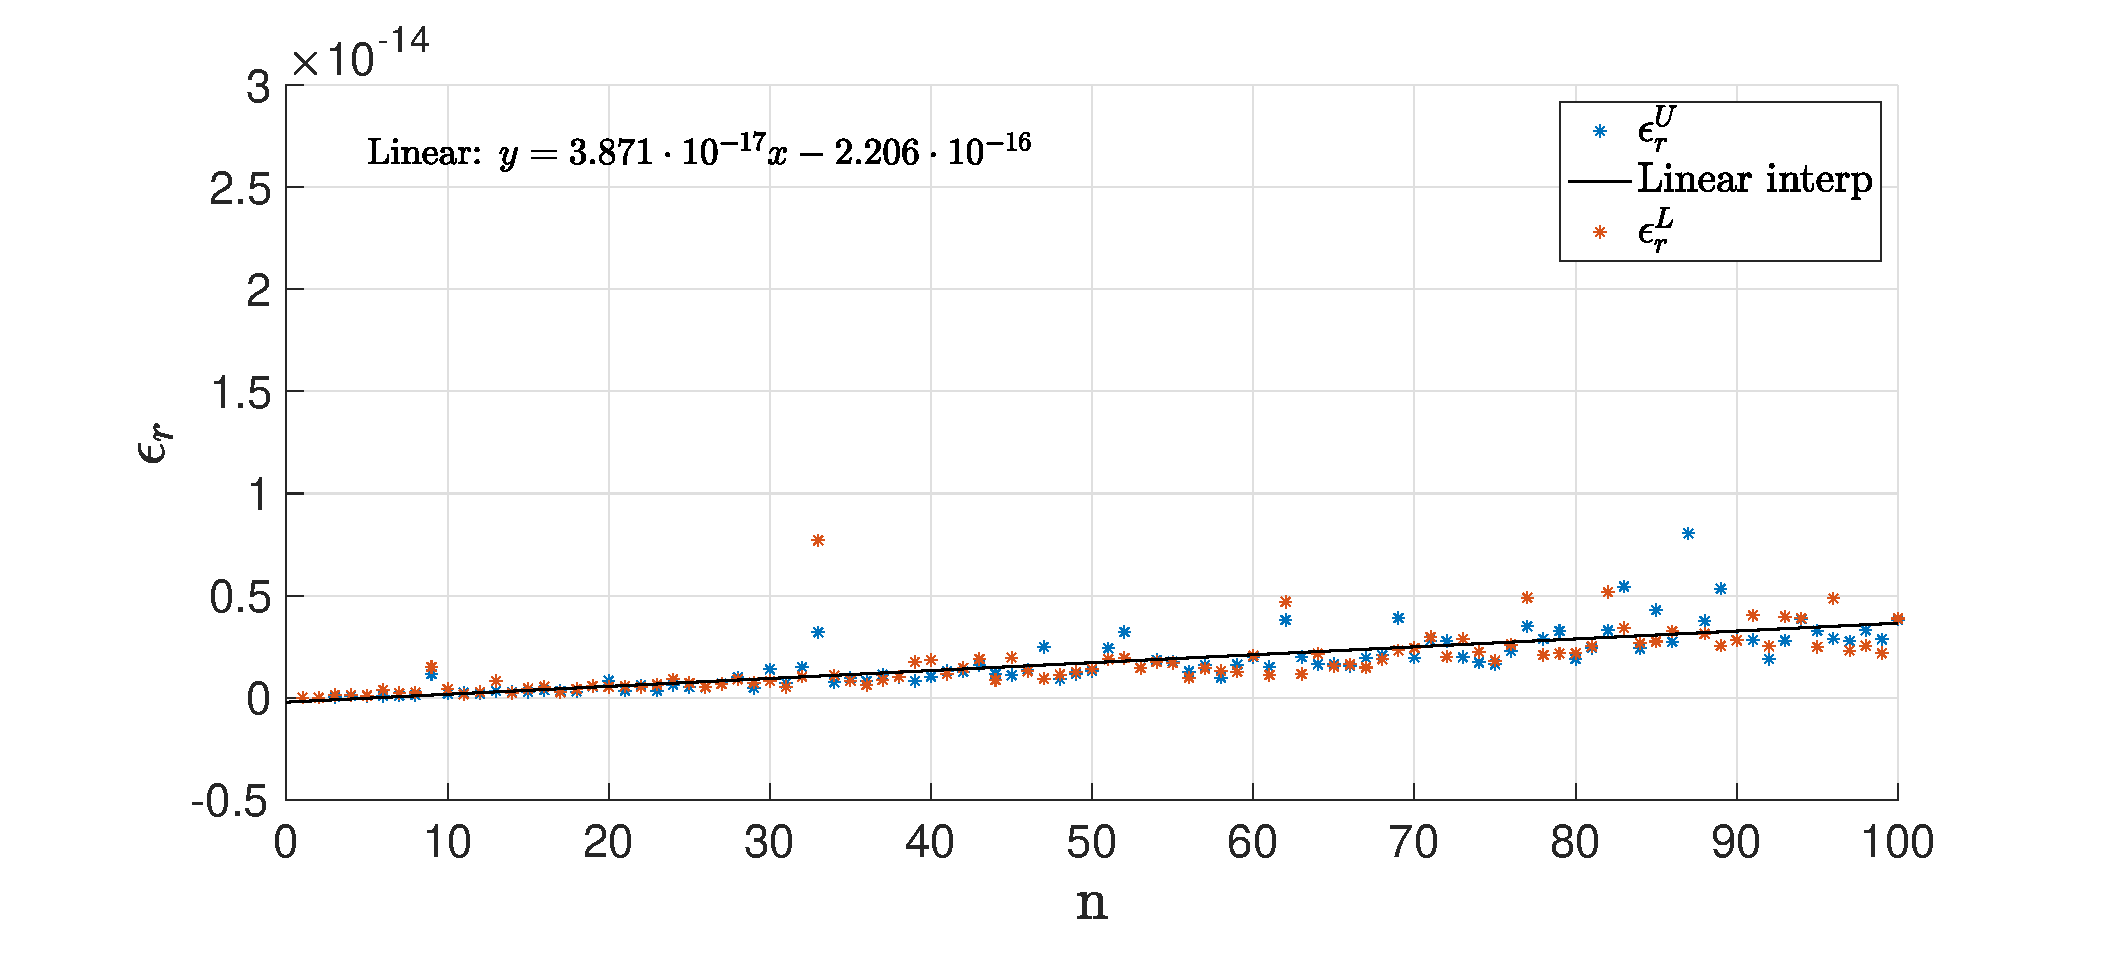
\includegraphics[width = 1 \textwidth]{LU_Err.eps}
	\caption{\label{LU_err}  Relative error on the values for the upper and lower triangular matrices obtained via our LU decomposition scheme, and Matlab's one. The subscripts U and L in the legend correspond to upper and lower triangular respectively.}
\end{figure}  

\end{homeworkSection}
\end{homeworkProblem}

%%%%%%%%%%%%%%%%%%%%%%%%%%%%%%%%%%%%%%%%%%%%%%%%
%%%%%%%%%%%%%%%%%%%%%%%%%%%%%%%%%%%%%%%%%%%%%%%%
\newpage

\begin{homeworkProblem}

\section{Equivalent resistance of infinite resistor grid}

Let us consider a grid of size $N\times (N-1)$ ($N$ odd) of resistors, all connected with their nearest neighbors, and all the same resistance of 1 $\Omega$ (see Fig.(\ref{grid})). In addition, the following quantities are defined according to the following convention: for $1\le i\le N$, $1\le j\le N-1$, $V(i,j)$ is the voltage measured at node $(i,j)$, $I_r(i,j)$ the current from node $(i,j)$ to node $(i+1,j)$ to the right and $I_t(i,j)$ the current from node $(i,j)$ to node $(i,j+1)$ above. Furthermore, open boundary conditions (B.C) are considered, i.e. no current can enter or flow out the system. Finally, the two points of interest are given by \\

\begin{gather}\label{points}
    A=\left(\frac{N-1}{2},\frac{N-1}{2}\right),\quad B=\left(\frac{N-1}{2}+2,\frac{N-1}{2}+1\right)
\end{gather}

\noindent and will be used to measure resistance. Indeed, a current of 1A is introduced at site A, while a current of 1A is extracted from the system at site B to ensure that the electrical current conservation.\\


\noindent Let us start by determining the number $N_u$ of unknowns, $V$, $I_r$ and $I_t$ as well as the number $N_c$ of constraints, given together by the boundary conditions, and Kirchoff's nodes law, and Ohm's law. An examination of Fig(\ref{grid}), with 5 nodes enabling an enumeration, it is possible to extrapolate this result to any $N_{nodes} =N$: \\

\begin{gather}
    N_u=3N(N-1),\qquad N_c=\underbrace{(N-1)^2+N(N-2)}_{\text{Ohm's law}}+\underbrace{N(N-1)}_{\text{Law of nodes}}+\underbrace{2N-1}_{B.C}
\end{gather}



\begin{figure}[H]
            \centering
            \includegraphics[scale=0.45]{grille.png} 
            \caption{\label{grid}Configuration for the problem described above}
 \end{figure}
\end{homeworkProblem}

\noindent In fact, take for example $N=5$. It follows that $N_u=3*5*4 =N_c=60$, so the problem could hopefully be solved by a matrix inversion. \\

\noindent Let us thus rewrite the system in a matrix form: $A\mathbf{x}=\mathbf{b}$, where $A$ is an $N_c\times N_u$ matrix, $\mathbf{x}$ a $N_u$-dimensional vector and $\mathbf{b}$ an $N_c$-dimensional vector. However, it appears (can be checked with Matlab), that the matrix $A$ is singular, that means non invertible. This result was physically expected. The voltages $V(i,j)$ are defined on each node of the mesh, but since a voltage is a potential difference, it needs to be measured between two nodes. Thus, the voltage is a translational invariant, in the sense that $\Delta V=V(i+1,j)-V(i,j)\equiv V(i+1+\delta x,j)-V(i+\delta x,j)$. Hence, an infinite number of voltage values can fit.\\

\noindent Thus, the kernel of $A$  has to be a 1-dimensional vector space. Matlab can provide an  orthonormal basis for the kernel of $A$ which is indeed a vector space of dimension 1 (one vector $\mathbf{v_0}$). Numerically, this can be verified since $A \cdot\mathbf{v_0} = \epsilon_m$, where $\epsilon_m$ is the machine precision epsilon ($\sim 0$).  \\

The way we decide to bypass this singular determinant problem is to project the problem on the orthogonal complement of $Ker(A)$. To do so, one needs the definition of a projection matrix $P_V$ of size $[N(N-1)+1]\times N(N-1)$ as follows:\\
 
\begin{gather}
P_V(V_1,V_2,...,V_N)=(V_2-V_1,V_3-V_1,...,V_N-V_1)
\end{gather}


\noindent The full projection matrix is a block diagonal matrix\\

\begin{gather}
P=
    \begin{pmatrix}
    P_V&0&0\\
    0&I&0\\
    0&0&I
    \end{pmatrix}
\end{gather}

\noindent where $I$ is a current matrix. It can be easily checked that $\det(PAP^t)\neq0$. The $P$ projection of the original system can be solved according to \\

\begin{gather}\label{system projection}
    PAP^t\mathbf{y}=P\mathbf{b},\qquad \mathbf{x}=P^t\mathbf{y}
\end{gather}

\noindent Now that $\mathbf{x}$ is known, one can obtain the value of the equivalent resistance $R_{\text{eq}}$ between $A$ and $B$ for any $N$.Note that the current entering the system in $A$ is fixed at 1A, and that the voltage between $A$ and $B$ varies, from Ohm's law, the equivalent resistance is computed to be: \\


\begin{gather}\label{req}   R_{\text{eq}}=V\underbrace{\left(\frac{N-1}{2},\frac{N-1}{2}\right)}_{\text{Point A}}-V\underbrace{\left(\frac{N-1}{2}+2,\frac{N-1}{2}+1\right)}_{\text{Point B}},\quad\forall N\quad\text{odd}
\end{gather}

\noindent Taking the particular case where $N=7$, using $\mathbf{x}$ obtained previously, it comes that $R_{\text{eq}}=0.8462$ $\Omega$.\\


\begin{figure}[H]
            \centering
            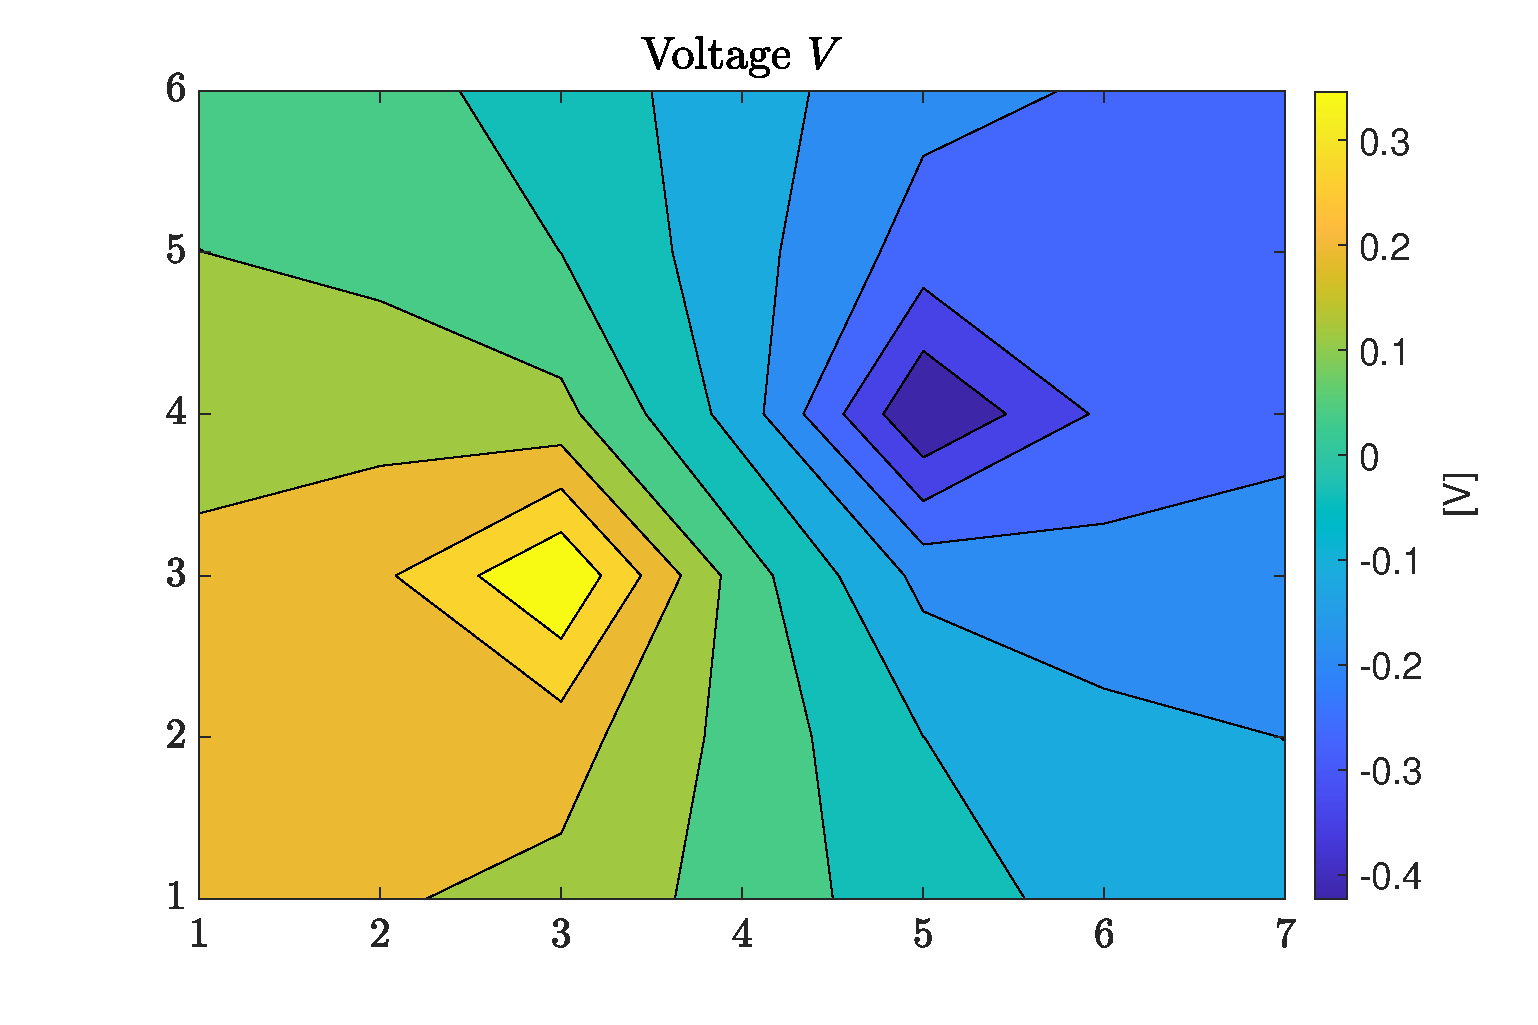
\includegraphics[scale=0.45]{voltage.eps} 
            \caption{\label{voltage}Voltage distribution along the grid $N=7$, $A=(3,3)$, $B=(5,4)$}
 \end{figure}
 
 The voltage and the currents $I_r$ and $I_t$ can be plotted, as in Fig.(\ref{voltage})-(\ref{It}). The voltage distribution is consistent with the expectations, since injecting a current in $A$ and extracting it in $B$ yields highest values in amplitude of voltage at those positions, in accordance with Ohm's law. The current distributions $I_t$ and $I_r$ are also consistent  with our initial assumptions. The boundary conditions are respected in the sense that no current can escape or enter the system.\\


\begin{figure}[H]
            \centering
            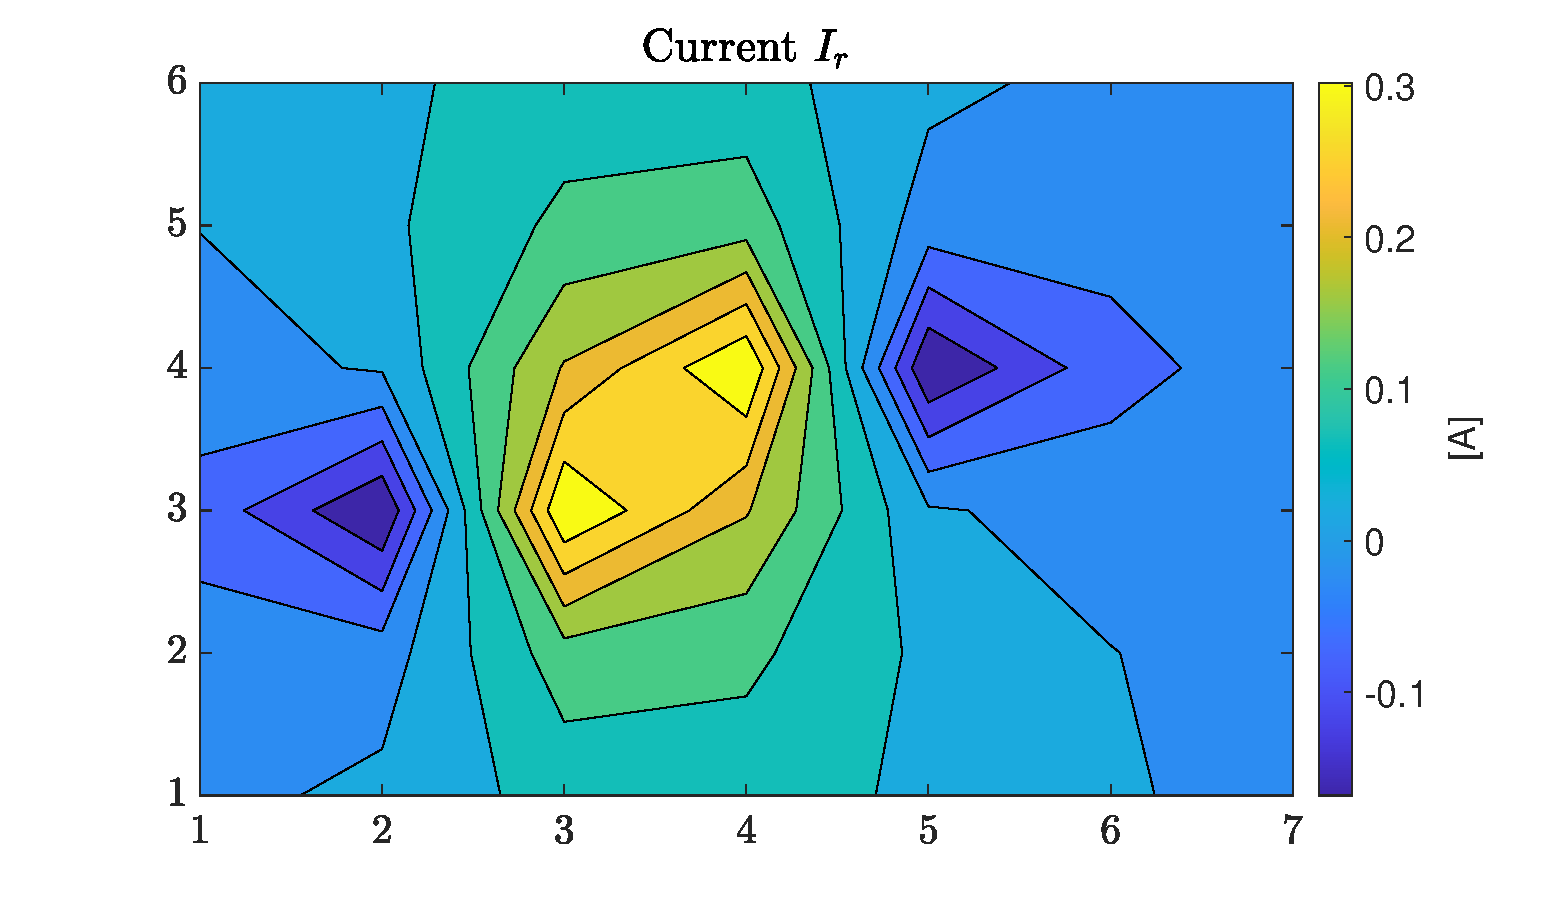
\includegraphics[scale=0.45]{Ir.eps} 
            \caption{\label{Ir}Current $I_r$ distribution for $N=7$}
 \end{figure}

\begin{figure}[H]
            \centering
            \includegraphics[scale=0.45]{It.eps} 
            \caption{\label{It}Current $I_t$ distribution for $N=7$}
 \end{figure}

\noindent Finally, it can be verified that Kirschoff's law of nodes holds, i.e. that the algebraic sum of the currents on a node is zero. To verify the law, the sum of the currents flowing in and out of each node can be plotted, as shown in Fig(\ref{kirchoff}). At points $A$ and $B$, the currents are indeed 1A and -1A, respectively. Elsewhere, the current is zero, as predicted.\\

\noindent Finally, let us study the convergence properties of the equivalent resistance $R_{\text{eq}}$ as a function of the size $N$ of the system. More precisely, the question is to determine what size $N$ of the system allows to reach an uncertainty smaller than $10^{-2}$ $\Omega$ on the equivalent resistance.\\

\begin{figure}[H]
            \centering
            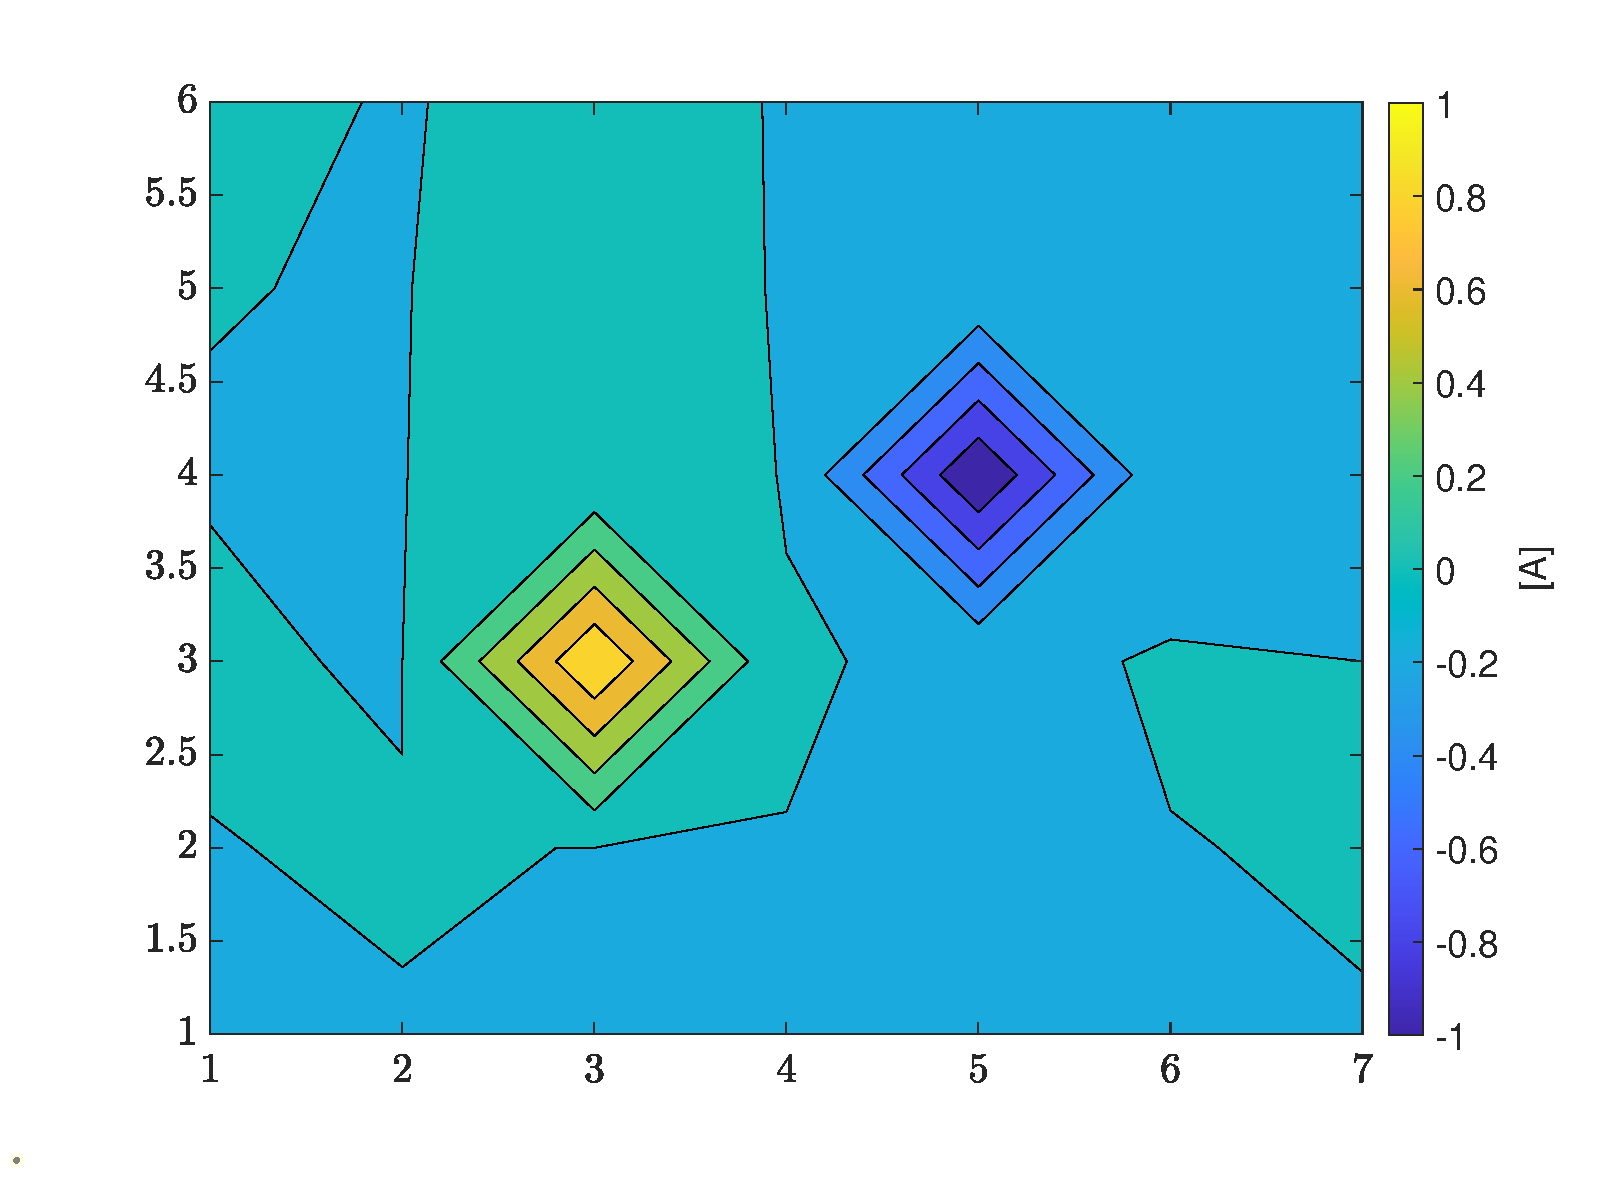
\includegraphics[scale=0.45]{Kirchoff.eps} 
            \caption{\label{kirchoff}}
 \end{figure}


\noindent In order to study the convergence, the size of the system is continuously increased, and the previously developed steps are repeated: generation of $A$ such that $A\mathbf{x}=\mathbf{b}$, generation of $P$ to project on the orthogonal complement of $Ker(A)$, solution of the system from Eq.(\ref{system projection}), and finally computation of the equivalent resistance using Eq.(\ref{req}). The result is shown in Fig.(\ref{convergence}). The minimum required size is $N=13$. \\

\begin{figure}[H]
            \centering
            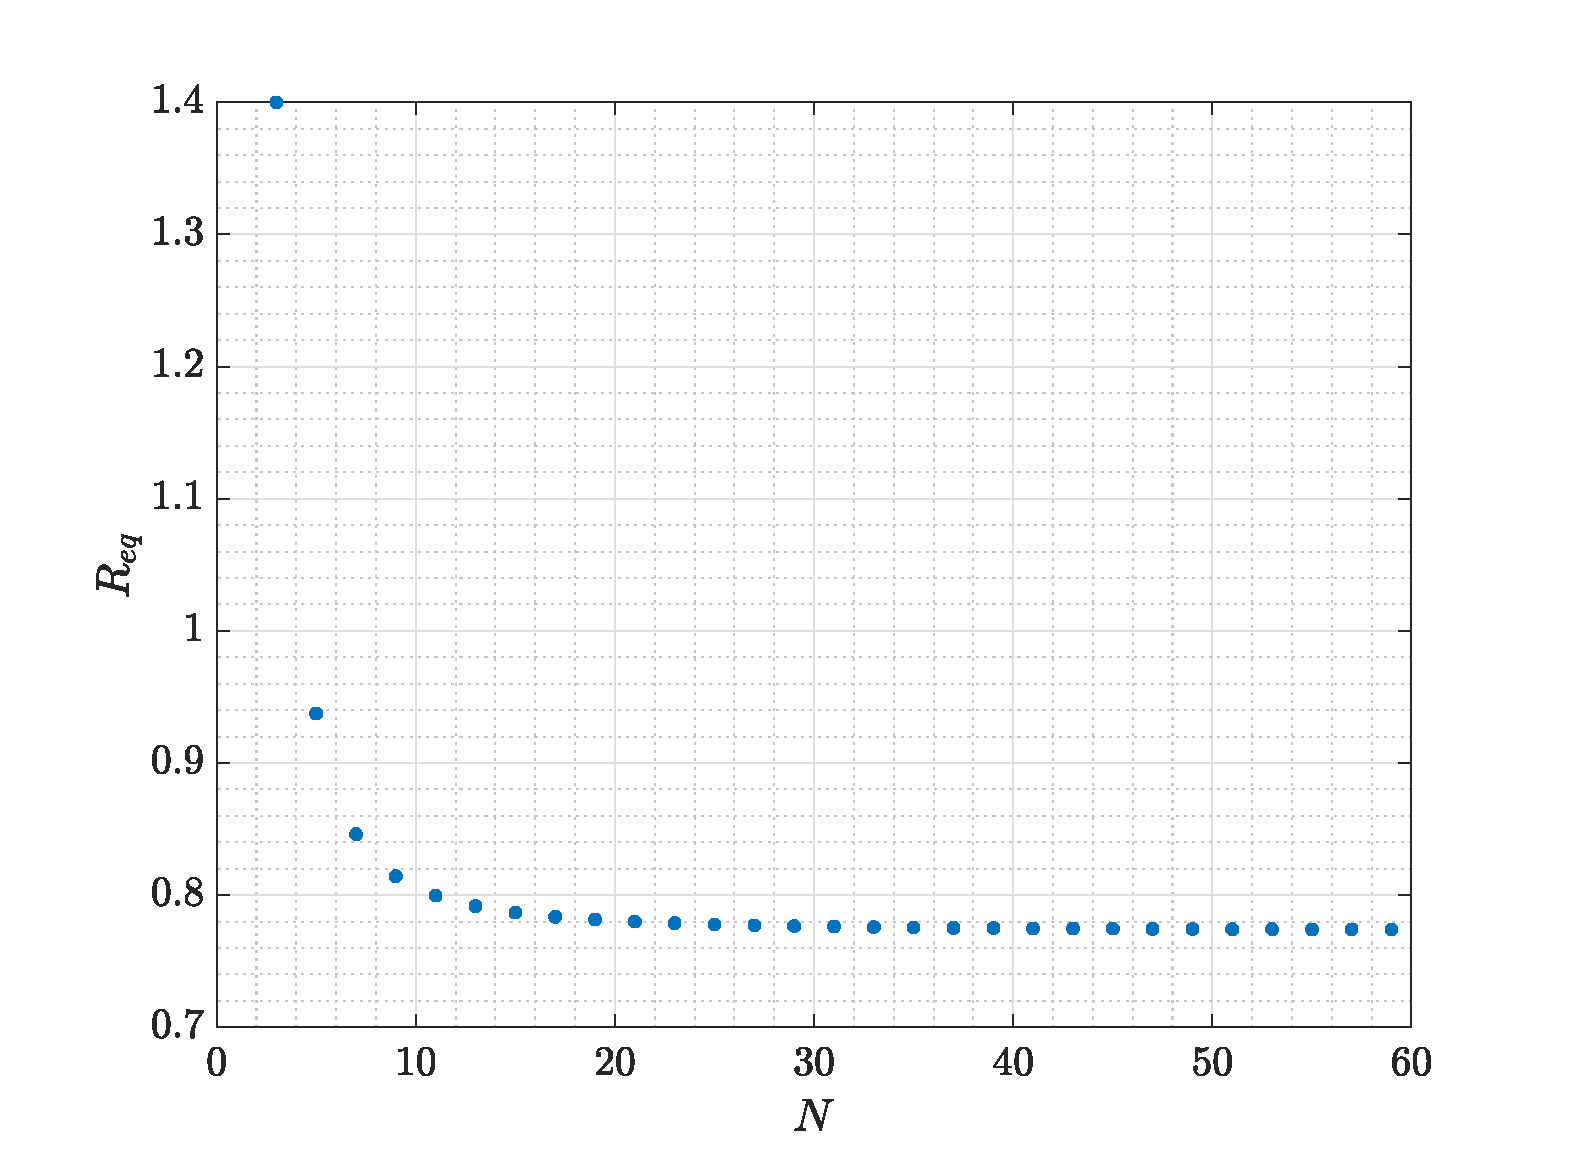
\includegraphics[scale=0.45]{convergence.eps} 
            \caption{\label{convergence}}
 \end{figure}
 
 \noindent Note that there exists an analytical solution for the same problem with an infinite grid, yileding $R_{\text{eq}}=4/\pi-1/2$. Thus, using the equivalent resistance obtained previously, an estimate of $\pi$ follows: $\pi\approx3.14$.\\
 
%%%%%%%%%%%%%%%%%%%%%%%%%%%%%%%%%%%%%%%%%%%%%%%%
%%%%%%%%%%%%%%%%%%%%%%%%%%%%%%%%%%%%%%%%%%%%%%%%
\newpage

\begin{homeworkProblem}

\section{Power iterations methods}

Iterative power methods provide solutions to eigenvalue problems by mean of algorithms giving sequences of approximate values that converge towards the true solutions of the eigenvalue problem. Usually, the complexity of the problem is of the order of $\mathcal{O}(mn^2)$ where $n$ is dimensionality of the problem and $m$ the number of iterations to reach the desired tolerance.\\

\noindent Here, we only detail the algorithm for the standard power method. A theoretical insight of inverse-power and Rayleigh quotient methods can be found in some literature as \cite{rayleigh}. The power method is based on the very straightforward principle of applying a matrix several times (hence to a certain power) till a certain tolerance is reached:\\

\begin{enumerate}
\item{Given the matrix $A$ for the eigenvalue problem, define a random unit vector $q^{(0)}$}
\item{The first element of the values sequence is $\lambda^{(0)} = q^{*(0)}Aq^{(0)}$, where $^*$ stands for the adjoint of the element}
\item{While $|\lambda^{(k)} - \lambda^{(k-1)}| > \epsilon$, where $\epsilon$ is the tolerance threshold, repeat the following:\\
	\begin{itemize}
	\item{$q^{(k)} = Aq^{(k-1)}$}
	\item{Normalize $q^{(k)}$}
	\item{$\lambda^{(k)} = q^{*(k)}Aq^{(k)}$}
	\end{itemize}
}
\item{Once the tolerance threshold is reached, $\lambda$ is retained as the last value of the above sequence.}\\
\end{enumerate}

\begin{homeworkSection}{1- Power method} 
	\matlabscript{simple3}{Matlab script for standard power method}
\end{homeworkSection}

\newpage
The documentation on how to use each function is included in each submitted script in the form \emph{MatlabScript.m} but has been removed here for the sake of saving space. However, each of them can be accessed upon typing the command \emph{help FunctionName} in the Matlab command line.\\

\noindent The inverse power method proceeds to a shift in the direction of the initial guessed eigenvalue, before performing the power iterations with the inverse of the shifted matrix.\\

\noindent The Rayleigh quotient method is very close to the inverse power method. The difference resides in the fact that the estimated eigenvalue is replace by the Rayleigh quotient at the end of each iteration.

\begin{homeworkSection}{2- Inverse power method} 
	\matlabscript{simple4}{Matlab script for inverse power method}
\end{homeworkSection}

\begin{homeworkSection}{3- Rayleigh quotient method} 
	\matlabscript{simple5}{Matlab script for the Rayleigh quotient method}
\end{homeworkSection}

\noindent All the tests from the scripts \emph{test$_{p,ip,rq}.m$} have been passed successfully.\\

\end{homeworkProblem}

%%%%%%%%%%%%%%%%%%%%%%%%%%%%%%%%%%%%%%%%%%%%%%%%
%%%%%%%%%%%%%%%%%%%%%%%%%%%%%%%%%%%%%%%%%%%%%%%%
\newpage

\begin{homeworkProblem}

\section{Vibrating modes of a string}

Considering a vibrating string, and denoting the amplitude of the vibrations by $u$, one gets that the amplitude will have the following dependence in space and time $u \equiv u(x,t)$. Introducing the constants $\kappa$ and $\rho$, corresponding respectively to energy and mass densities per unit length, the action of the problem in the harmonic approximation reads:\\

\beq
\S[u(x,t)] = \int_{t_1}^{t_2}dt \int_{0}^{L}dx \Bigg( \frac{1}{2}\rho \Big(\frac{\partial u}{\partial t}\Big)^2- \frac{1}{2}\kappa \Big(\frac{\partial u}{\partial x}\Big)^2\Bigg).
\eeq \\

\noindent Taking the first variation of the action yields to the following Euler-Lagrange equation, namely the wave equation: \\

\beq
\frac{\partial^2 u}{\partial t^2} = \frac{\kappa}{\rho}\frac{\partial^2 u}{\partial x^2}.\label{wave}
\eeq\\

\noindent Applying the following ansatz to decouple the space and time dependences $u(x,t) :=v(t)w(x)$, one gets, plugging it in in Eq.(\ref{wave}),\\

\beq
\frac{v''}{v} = \frac{\kappa}{\rho}\frac{w''}{w},
\eeq\\

\noindent where $''$ represents the second order derivative w.r.t the variable it depends on. Since the left term depends on time and the right term depends on space, both terms have to be constant, so focusing on the space term $w''/w$, one gets that\\

\beq
\frac{w''}{w}\frac{\kappa}{\rho} = c \implies w'' = -\lambda w\label{new_wave},
\eeq\\

\noindent where $\lambda = -c\rho/\kappa$. Lambda has the units of $m^{-2}$, which corresponds to the a wave vector squared. If we want to avoid the trivial solution $w\equiv0$, one has to impose $\lambda \neq 0$. Delving a bit more in the analytical structure of the solutions of Eq.(\ref{new_wave}), one sees that the solution need to be such that there exists a set of integers $k$ such that $\lambda \propto k^2/L^2$. In fact, the general solution of Eq.(\ref{new_wave}) can be expressed as:\\

\beq
w(x) = A\cos(\sqrt{\lambda}x) + B\sin(\sqrt{\lambda}x),
\eeq\\

\noindent with $A$ and $B$ real valued amplitudes. Together with Dirichlet boundary conditions, one notices that $A$ has to vanish, and that $\lambda = (k\pi/L)^2$, with $k$ non-zero integers.\\

\newpage
\noindent  To solve this equation, the second order space derivative from Eq.(\ref{new_wave}) can be numerically implemented using centered finite differences, having discretized space with $N$ points. Hence, together with the minus term in front of $\lambda$, the latter can be rewritten as an eigenvalue problem:\\

\beq
A \mathbf{w} = \lambda \mathbf{w},
\eeq\\

\noindent where the $N\times N$ matrix $A$ is defined as follows:\\

\beq
A = \Big(\frac{N-1}{2}\Big)^2\left(\begin{array}{cccccc}2 & -1 & 0 & 0 & …& 0 \\-1 & 2 & -1 & … &0& 0 \\0 & -1 & 2 & -1&0 & 0 \\ 0 & … & … & … & … & 0 \\0 & 0 & … & -1 & 2 & -1 \\0 &  0 & 0 & … & -1 & 2\end{array}\right)
\eeq\\

\noindent An obvious comment can be done about the structure of $A$, that gives out information about the nature of the eigenvalues of $A$: it is tridiagonal and such that $A^{T}=A$. So since $A$ is an orthogonal matrix, there exists a basis of eigenvectors in which $A$ can be diagonalized. Moreover, the eigenvalues are strictly positive, and can be ordered, such that they correspond to different 'energy states' of the vibratory system. As of the vector $\mathbf{w}$, since we chose Dirichlet boundary counditions $u(0,t) = u(L,t)$ $\forall t$, one gets that $w_1 = w_N = 0$. The scalar factor in front of the matrix corresponds to $1/dx^2$, where $dx$ is the distance between two meshpoints. Since for $N$ mesh points, one has $N-1$ intervals, the length of one interval is $dx = L/(N-1) = 1/(N-1)$ in our context. \\

\noindent Now that the problem has been discretized, it is possible to find the lowest eigenvalue $\lambda_0$ with the inverse power method that we implemented in the previous part of the report, using a zero shift ($\mu = 0$). The numerically obtained value is $\lambda_0 = 9.7909$ m$^{-2}$. The corresponding vibrating eigenmode is plotted in Fig.(\ref{lowest_eigenmode}).\\


\begin{figure}[h!]
\centering
	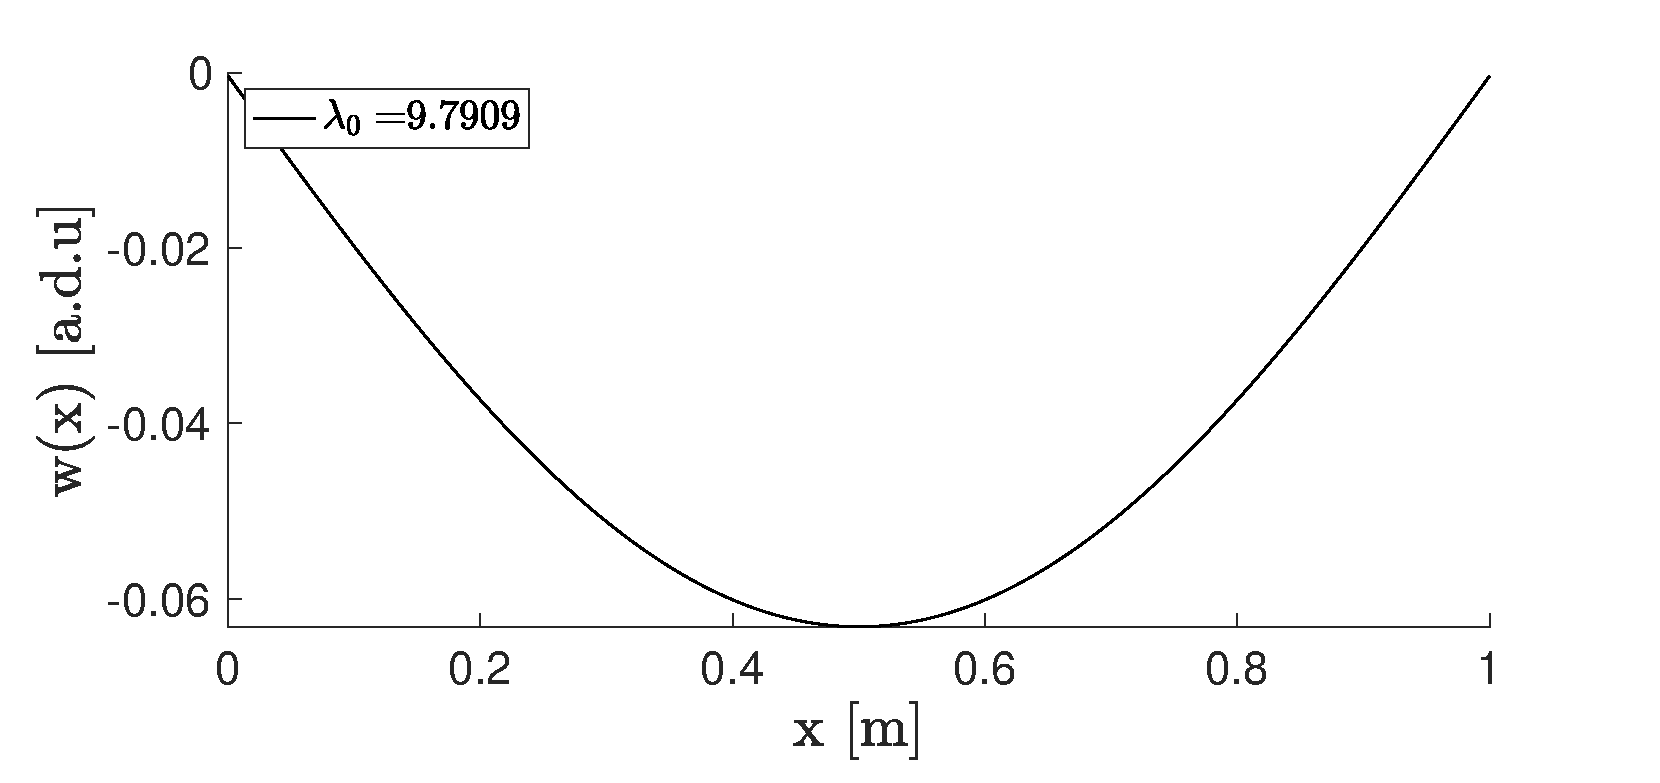
\includegraphics[width = 0.8 \textwidth]{lower_eigen.eps}
	\caption{\label{lowest_eigenmode}  Eigenmode for lowest eigenvalue $\lambda_0$.}
\end{figure} 

\noindent Note that the result corresponds to the first standing wave mode for a rope with Dirichlet boundary conditions. In Fig.(\ref{lowest_eigenmode}), [a.d.u] means arbitrary distance unit, since the units depends on the discretization of the problem and haven't been normalized here.\\  

\noindent Now that the lowest eigenvalue has been found, we can focus on higher eigenvalues. To do so, we use the inverse power method with a non-zero shift, and the shift is chosen, for each order, to be the values $\lambda_n := (n^2\pi^2/L^2)$. One notes that the first eigenmode for $\lambda_1$  is identical to the mode $\lambda_0$. For higher orders, that is higher values of $n$, we recover the usual standing wave modes, as pictured in Fig.(\ref{standing_modes}). 
 
\begin{figure}[h!]
\centering
	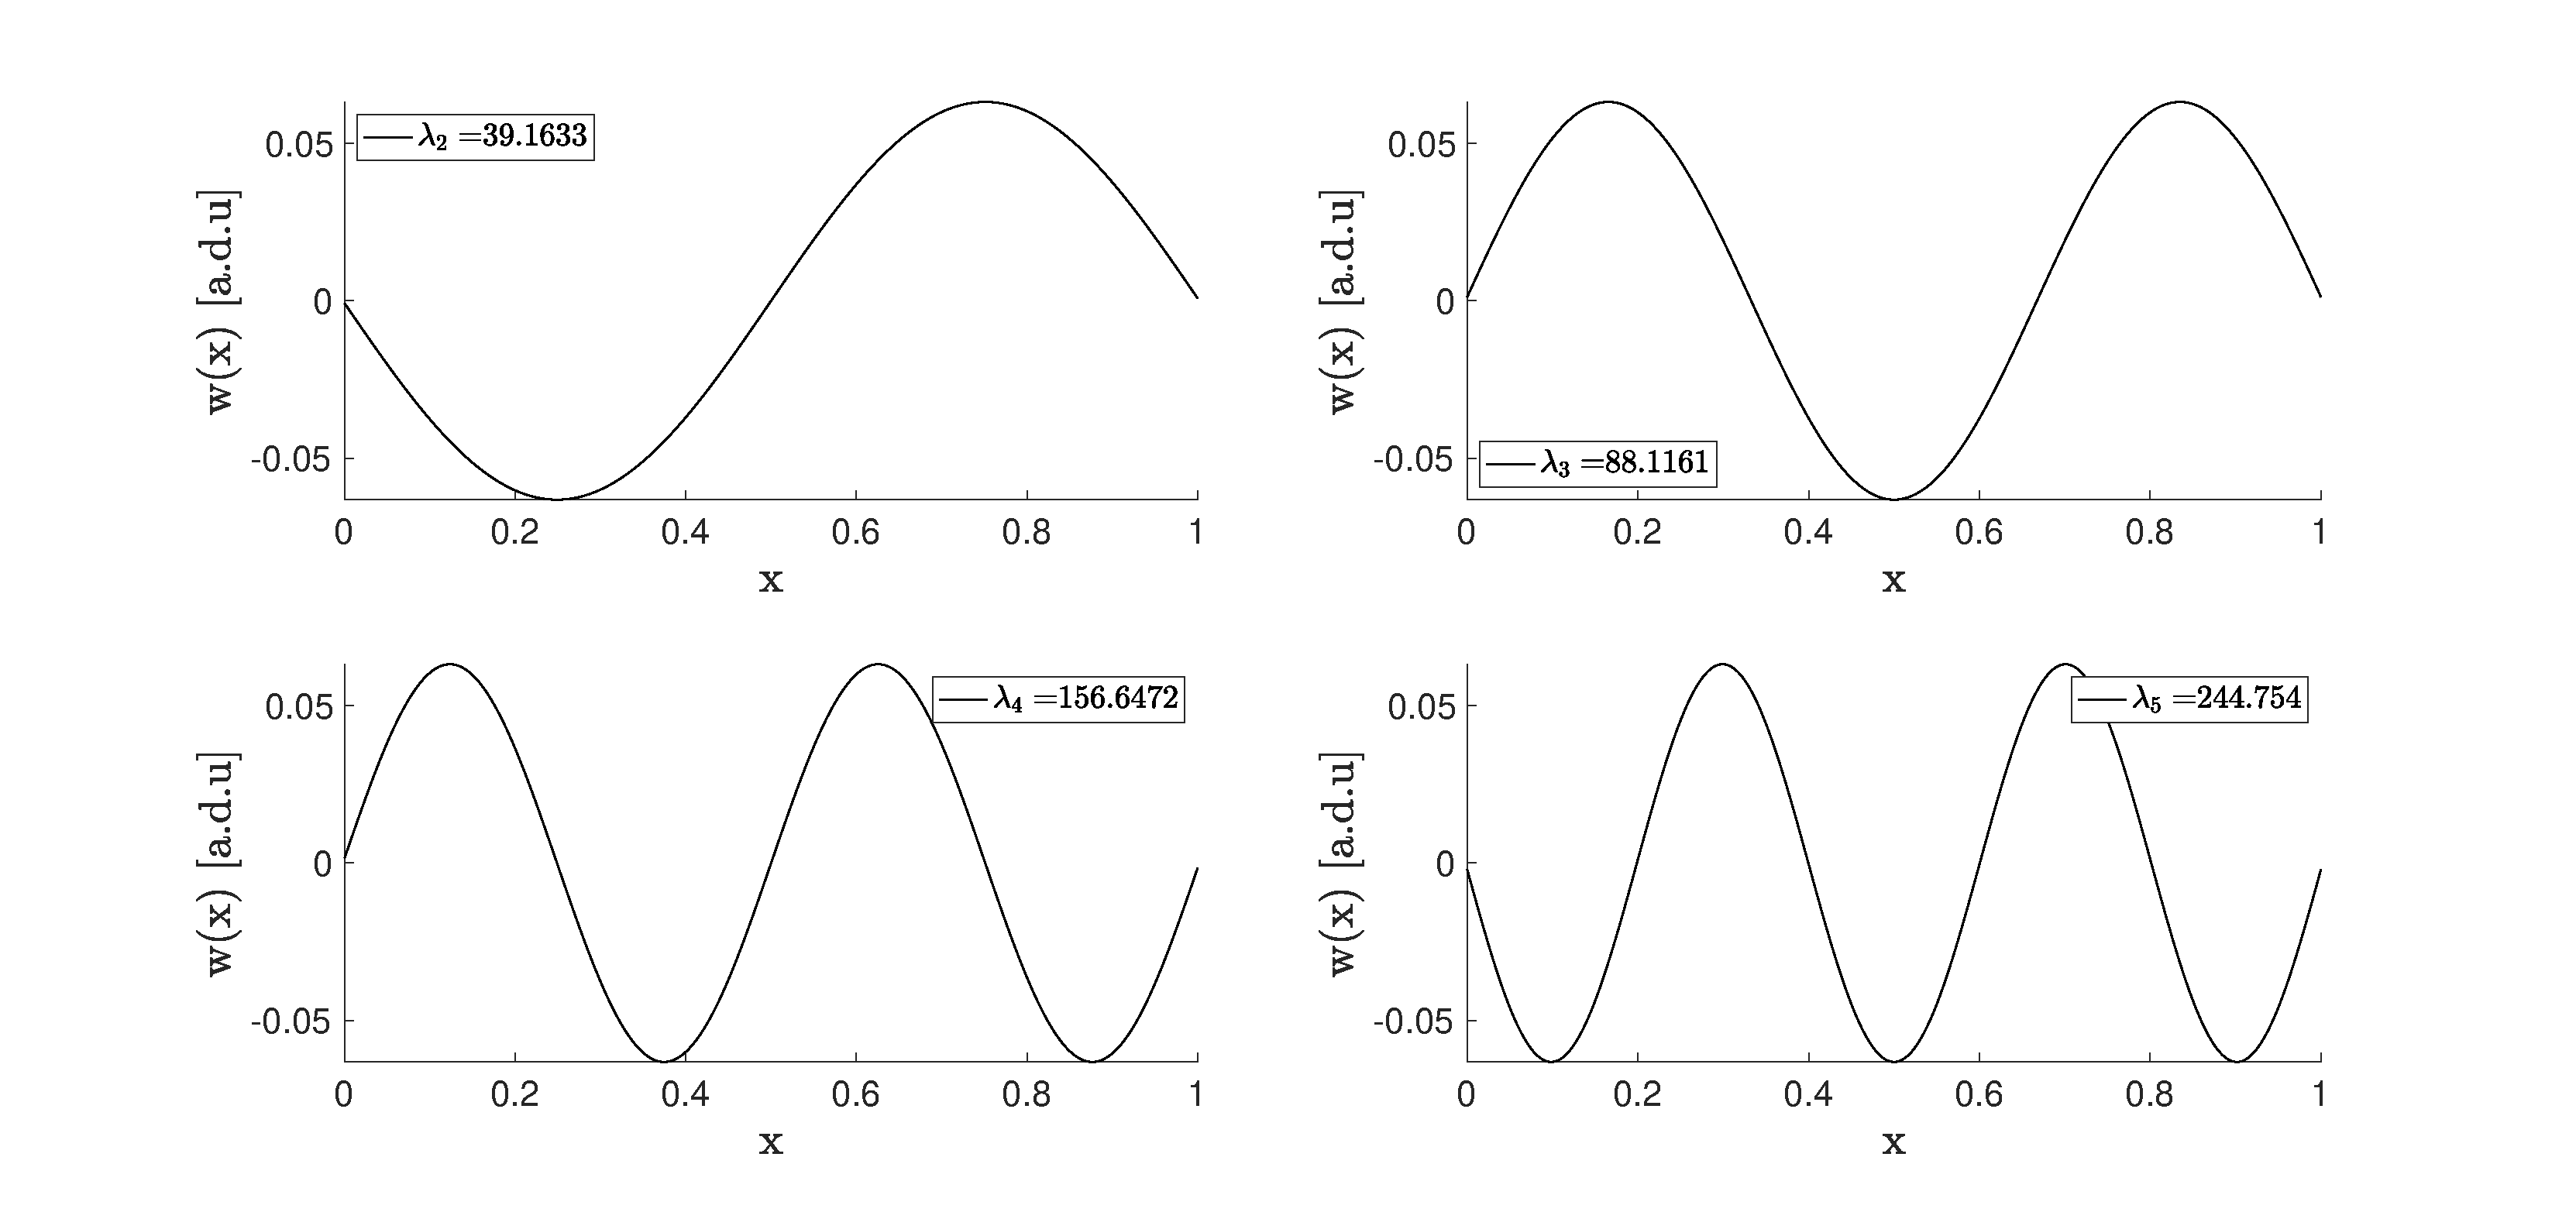
\includegraphics[width = 1. \textwidth]{eigenmodes}
	\caption{\label{standing_modes} The four lowest values modes above the ground state $\lambda_0$. Note that $n$ from $\lambda_n$ is the number of peaks from each standing wave profile. }
\end{figure} 

\noindent One will note that the eigenvalues here have been found with inverse power method with shift, assuming that the the eigenvalue were known to be the values $\lambda_n$ from the solution of the wave differential equation. In fine, the method worked pretty well, because a comparison of the analytical $\lambda_n$ and the numerically obtained values shows low error, as in Tab.(\ref{table}).\\

\begin{table}[H]
    \centering
    \begin{tabular}{|c|c|c|c|c|c|}
    \hline Eigenvalues [m$^{-2}$] & $\lambda_1$ & $\lambda_2$ & $\lambda_3$ & $\lambda_4$ & $\lambda_5$ \\
    \hline Analytical & 9.8696 & 39.4784 & 88.8264 & 157.9137 & 246.7401\\
    \hline Numerical & 9.7909 & 39.1633 & 88.1161 & 156.6472 & 244.7540 \\
    \hline 
    \end{tabular}
    \caption{Comparison between the eigenvalues obtained analytically and numerically.}
    \label{table}
\end{table}


\end{homeworkProblem}



%%%%%%%%%%%%%%%%%%%%%%%%%%%%%%%%%%%%%%%%%%%%%%%%
%%%%%%%%%%%%%%%%%%%%%%%%%%%%%%%%%%%%%%%%%%%%%%%%




\newpage

\begin{homeworkProblem}

\section{Jacobi Method}

Though effective, using the power iterative methods can be problematic as they only allow to determine one eigenvalue at a time. A more efficient way would be to diagonalize the matrix from the eigenvalue problem, which corresponds to finding an eigen-basis in which the matrix is diagonal, with its diagonal elements corresponding to the eigenvalues. In the following, we give two implementations of the Jacobi method, the second being the cyclic Jacobi algorithm, which supposedly performs way less rotations to diagonalize the matrix. A comparison of the two algorithms will be presented after the scripts are introduced.\\

\noindent The matrices treated by the Jacobi methods must be symmetric $N\times N$ matrices. The main idea behind these methods, implemented in the algorithms \verb|eig_j.m| (Jacobi method) and \verb|eig_cj.m| (cyclic Jacobi method), is to reduce the norm of the off-diagonal elements of the matrix $A$, define as off$(A)=(\sum_{i,j,i\neq j}a_{i,j}^2)^{1/2}$.


\subsection{Jacobi \& cyclic Jacobi method}
Let us explain in more details how both these two methods work. First, it is a matter of identifying the off-diagonal element with the highest amplitude, i.e. finding $(i,j)$ such that $|a_{i,j}|=\max_{l\neq m}|a_{m,n}|$. Once this pair is determined, the Jacobi matrix $J_{ac}$ can be constructed before performing a Jacobi rotation on the matrix $A$ until a certain tolerance is reached.  Note however the high computational cost of finding the largest off-diagonal elements, since running through both the rows and the columns can only be done in $\mathcal{O}(n^2)$.\\

\noindent The cyclic Jacob method can drastically reduce the computational cost. Instead of finding the largest off diagonal elements, the method consists in running through the rows.The operating cost of this method is about $\mathcal{O}(n^3\log(\log(|\epsilon|)))$, where $\epsilon_m$ is the machine precision.\\

\noindent In order to compare the efficiency of the two methods, the computational time needed to diagonalize random matrices of increasing size is plotted on the left part of Fig.(\ref{jacobi_fig}), for both the standard and the cyclic Jacobi algorithms. On the right part of Fig.(\ref{jacobi_fig}), it is the number of rotations required to perform the diagonalization which is represented. One immediately notices that the cyclic Jacobi is much more efficient.\\


\begin{figure}[h!]
\centering
	\includegraphics[width = 1 \textwidth]{Jacobi.eps}
	\caption{\label{jacobi_fig}  Left: Computational time for both cyclic Jacobi (red) and standard Jacobi (blue) methods - Right: same for the number of rotations.}
\end{figure}  

\end{homeworkProblem}

%%%%%%%%%%%%%%%%%%%%%%%%%%%%%%%%%%%%%%%%%%%%%%%%
%%%%%%%%%%%%%%%%%%%%%%%%%%%%%%%%%%%%%%%%%%%%%%%%



\newpage

\begin{homeworkProblem}

\section{2D quantum well}

Let us represent a two-dimensional elliptical quantum well by the following potential, where $V_0<0$ is constant, and the ellipticity is set via the parameter $c$. In our numerical implementation, we'll choose $V_0=-1.5$ eV and $r=1$ nm.\\

\beq
V(x)=
\begin{cases}
    V_0<0,&\quad x^2+y^2/c^2<r^2\\
    0,&\quad \text{otherwise}
\end{cases}
\eeq\\

\noindent The electrons moving inside the potential well are described by the time-independent Schrödinger equation, where $\hat{\mathcal{H}}$ is the hamiltonian of the system, $\psi$ and $E$ respectively the wave-function and the energy of the particle:\\

\beq
\hat{\mathcal{H}}\psi := -\frac{\hbar^2}{2m_e}\Delta\psi + \hat{V}\psi = E \psi, \label{Schro}
\eeq\\

\noindent where we denoted by $m_e$ the electron mass, $\hbar$ is the reduced Planck constant and $\Delta$ the Laplace operator. On the 2D cartesian coordinates, the Laplace operator takes the form $\Delta := \partial^2/ \partial x^2 + \partial^2/ \partial y^2$. As of the implementation, defining a cartesian grid with $N\times N$ points, $\psi$ and $V$ can both be represented as matrices. The values of the matrix associated to $\psi$ will evolve according to Eq.(\ref{Schro}) whereas the potential matrix will be fixed. Denoting $\psi(x_i,y_j) = \psi_{i,j}$ and $V(x_i,y_j) = V_{i,j}$, the discretized Schrödinger equation reads:\\

\beq
-\frac{\hbar^2}{2m_e}\Delta\psi_{i,j} + V_{i,j}\psi_{i,j} = E\psi_{i,j}. \label{Schro_disc}
\eeq\\

\noindent Now using centered finite differences to implement the Laplace operator, that is\\

\beq
\begin{split}
\frac{\partial^2 \psi}{\partial x^2} &= \frac{1}{(\Delta x)^2}\big(\psi_{i-1,j}- 2\psi_{i,j} + \psi_{i+1,j}\big)\\
\frac{\partial^2 \psi}{\partial y^2} &= \frac{1}{(\Delta y)^2}\big(\psi_{i,j-1}- 2\psi_{i,j} + \psi_{i,j+1}\big)\\
\end{split}
\eeq\\

\noindent so Eq.(\ref{Schro_disc}) can finally be recast as\\

\beq
\begin{split}
&-\frac{\hbar^2}{2m_e}\Bigg\{ -2 \Big( \frac{\Delta x^2 + \Delta y^2}{\Delta x^2 \Delta y^2}\Big)\psi_{i,j} + \frac{1}{\Delta x^2}\Big(\psi_{i-1,j}+ \psi_{i+1,j} \Big)+ \frac{1}{\Delta y^2}\Big(\psi_{i,j-1}+ \psi_{i,j+1} \Big)\Bigg\}\\
+&V_{i,j}\psi_{i,j} = E \psi_{i,j}\\
\end{split}
\eeq

\begin{figure}[h!]
\centering
	\includegraphics[width = 0.6 \textwidth]{Hamiltonian.eps}
	\caption{\label{hamiltonian}  Representation of our hamiltonian operator as a sparse matrix - $c=1$}
\end{figure}  

\noindent Fig.(\ref{hamiltonian}) shows the representation of our hamiltonian operator as a sparse matrix. Each blue dot represents a non zero coefficient, acting on the $(1\times N^2)$ vector containing each grid point. The diagonal corresponds to the Laplacian term, and the circle to the potential region. Fig.(\ref{hamilton_ellipt}) shows the same for a non zero ellipticity, that is for a parameter $c=2\neq 1$.\\

\begin{figure}[h!]
\centering
	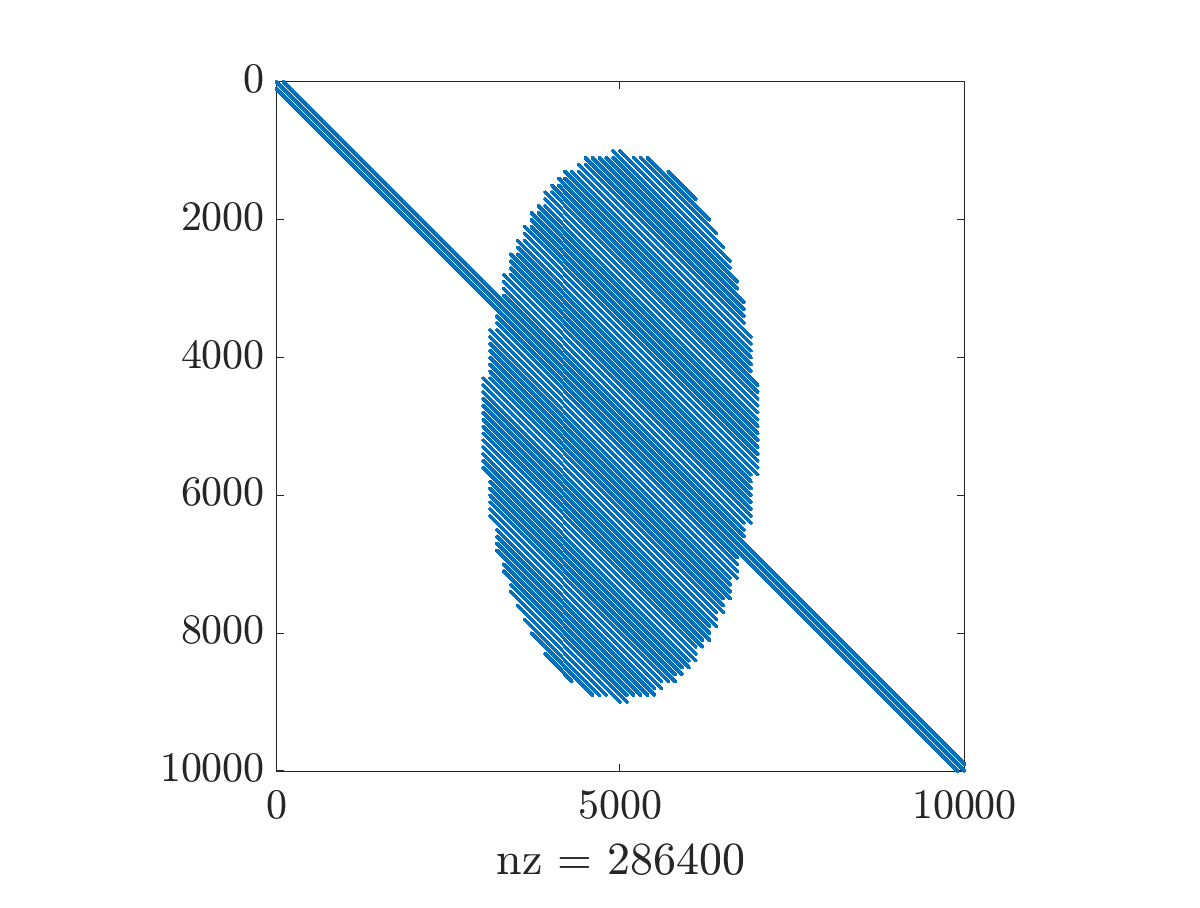
\includegraphics[width = 0.6 \textwidth]{Hamiltonian_ellipt.eps}
	\caption{\label{hamilton_ellipt}  Representation of our hamiltonian operator as a sparse matrix - $c=2$}
\end{figure}  
\end{homeworkProblem}

%%%%%%%%%%%%%%%%%%%%%%%%%%%%%%%%%%%%%%%%%%%%%%%%
%%%%%%%%%%%%%%%%%%%%%%%%%%%%%%%%%%%%%%%%%%%%%%%%
\newpage




\end{spacing}

\newpage
\bibliographystyle{alpha}
\bibliography{references}
\end{document}
\end{document}

%%%%%%%%%%%%%%%%%%%%%%%%%%%%%%%%%%%%%%%%%%%%%%%%%%%%%%%%%%%%%
